\documentclass[20pt]{article}
\usepackage{graphicx}
\usepackage{blindtext}
\usepackage{subfiles}
\usepackage[utf8]{inputenc}
\usepackage[russian]{babel}
\usepackage{setspace, amsmath}
\usepackage{array}
\usepackage{amssymb}

\graphicspath{{images/}}

\title{
    \textbf{Подготовка к экзамену по дисциплине «Математическая логика и теория алгоритмов»
    }
}
\author{Преподаватель: Моргунов В. М\\
        Студент: Дьяченко С. С\\
}

\begin{document}
    \maketitle
	\begin{figure}[th]
		\centering
		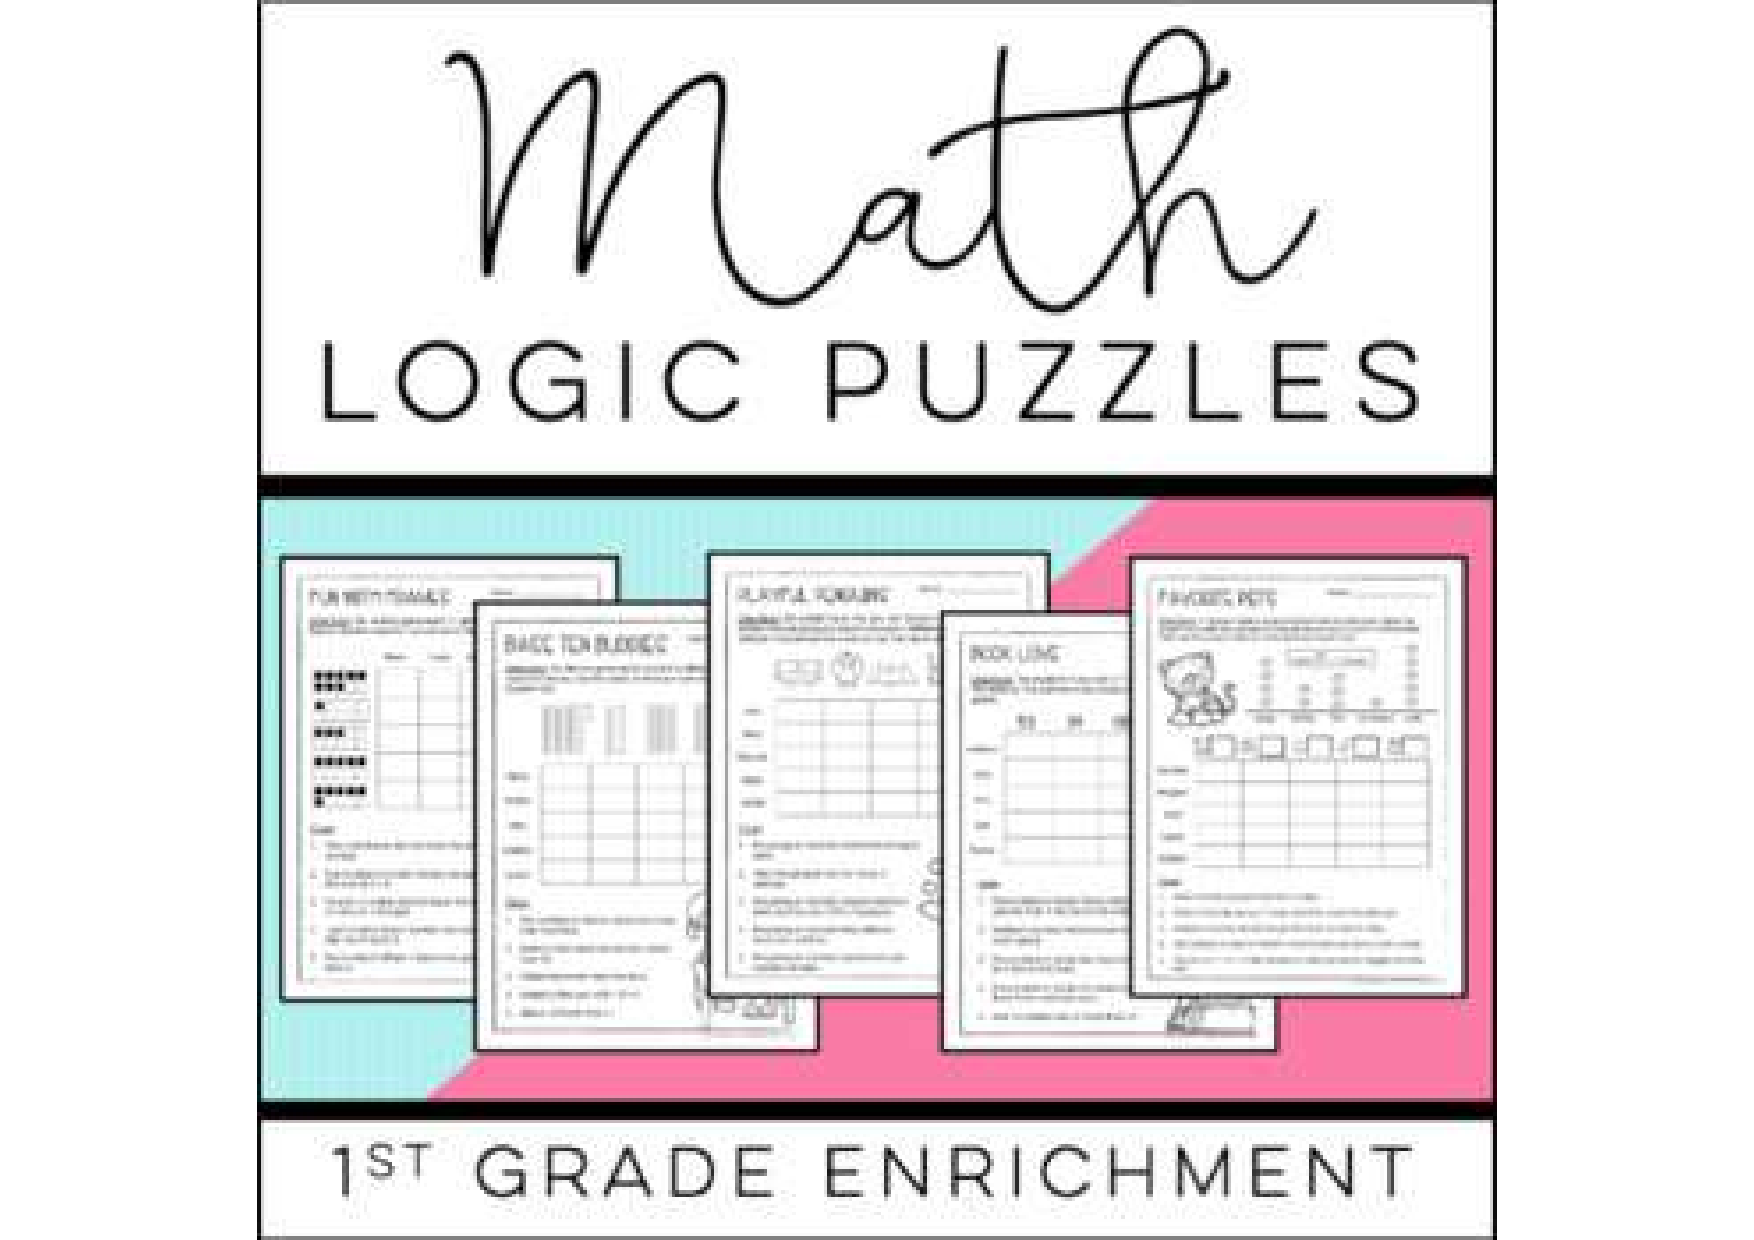
\includegraphics[width=7cm]{overleaf-logo}
		\label{fig:img1}
	\end{figure}

	\subfile{sections/section1} % Сектор логики высказываний 1 - 15
	\subfile{sections/section2} % Сектор ФИВ 16 - 19
	\subfile{sections/section3} % Сектор логики предикатов 20 - 27
	\subfile{sections/section4} % Сектор ФИП 28 - 29
	\subfile{sections/section5} % Сектор ФА 30 - 38
	\subfile{sections/section6} % Сектор МТ 39 - 44
	\subfile{sections/section7} % Сектор функции 44 - 50
	\subfile{sections/section8} % Сектор алгоритма 51 - 60

\end{document}